\documentclass[a1,landscape]{a0poster}
\usepackage{multicol} % This is so we can have multiple columns of text side-by-side
\columnsep=30pt % This is the amount of white space between the columns in the poster
\columnseprule=1 pt % This is the thickness of the black line between the columns in the poster
\usepackage{relsize}
\usepackage[svgnames]{xcolor} % Specify colors by their 'svgnames', for a full list of all colors available see here: http://www.latextemplates.com/svgnames-colors
\usepackage{relsize}
%\usepackage{times} % Use the times font
\usepackage{palatino} % Uncomment to use the Palatino font
\usepackage{framed}
\usepackage{graphicx} % Required for including images
\usepackage[font=small,labelfont=bf]{caption} % Required for specifying captions to tables and figures
\usepackage{amsfonts, amsmath, amsthm, amssymb} % For math fonts, symbols and environments
\usepackage{wrapfig} % Allows wrapping text around tables and figures
\usepackage{tikz-cd}
\usepackage{url}
\usepackage{float}
\newtheorem{definition}{Definition}[section]
\newtheorem{lemma}{Lemma}[section]
\newtheorem{theorem}{Theorem}[section]
\newtheorem{corollary}{Corollary}[section]
\newtheorem{proposition}{Proposition}[section]
\renewcommand\qedsymbol{$\blacksquare$}
\usepackage{tcolorbox}
\usepackage{lipsum}
\tcbuselibrary{skins,breakable}
\usetikzlibrary{shadings,shadows}
\newenvironment{myexampleblock}[1]{%
    \tcolorbox[beamer,%
    noparskip,breakable,
    colback=LightGray,colframe=LightGray,%
    colbacklower=LightGray!75!LightGray,%
    title=#1]}%
    {\endtcolorbox}
\begin{document}
\relscale{0.5}
%----------------------------------------------------------------------------------------
%	POSTER HEADER 
%----------------------------------------------------------------------------------------

% The header is divided into three boxes:
% The first is 55% wide and houses the title, subtitle, names and university/organization
% The second is 25% wide and houses contact information
% The third is 19% wide and houses a logo for your university/organization or a photo of you
% The widths of these boxes can be easily edited to accommodate your content as you see fit
\begin{minipage}[b]{0.9\linewidth}
\Huge \color{NavyBlue}{\textbf{Sleepbot - examining generalization error}} \color{Black}\\ % Title
\large \textbf{Dhasharath Shrivathsa, Yuzhong Huang}\\ % Author(s)
\large \textit{Computational robotics - Spring '17}\ % University/organization
\end{minipage}


\vspace{1cm} % A bit of extra whitespace between the header and poster content

%----------------------------------------------------------------------------------------

\begin{multicols}{4} % This is how many columns your poster will be broken into, a poster with many figures may benefit from less columns whereas a text-heavy poster benefits from more

\begin{abstract}
	Sleepbot is our project for improvements in generalization error for convolutional neural networks. Inspired by neuroscience, we aimed to build heuristics to speed up training or improve test set performance.
	We built visualization, logging, graphing, and statistics for a CNN to this effect.
	The structure of our code allows training processes to be transferred to some extent, through training a secondary network around the training process, though we did not thouroughly investigate this.
\end{abstract}
\color{NavyBlue}
\small
\part*{Problem framing} 
	\color{Black}
	\section*{Generalization error in Neural networks}
				\paragraph{Background}
				Initially inspired by neuroscience\cite{hobson2002cognitive}, deep learning have achieved great results in various research area including Computer Vision, Natural Language Processing and Robot Controls. Driven by the demand for high speed performance, most deep learning frameworks are confined to a layer-based form, which is efficient and compatible with the current computing system.\cite{krizhevsky2012imagenet}
				There is merit to changing this architecture, as evidenced by \cite{harvey2003skipnet}, and one way is to take a critical look at backpropogation.
        \paragraph{The training process} - \\
        Convolutional neural networks are trained by
        \begin{enumerate}
        	\item Feedforward a batch of images (a tunable "chunk" of the dataset)
        	\item Backpropogate the errors of the collective batch
        	\item Repeat for $n$ epochs
        \end{enumerate}
	      In the middle is the most important step, what is considered "training". Backpropogation calculates the error magnitude for each neuron and updates it's weights in closed form.
	      Our method intercepts weights in between training batches, so between each step of backpropogation.
	      \paragraph{Backpropogation}
	      What is wrong with backpropogation? It is a formative algorithim, used to propogate weight update throught the network. Unfortunatley, its biggest strength is also its biggest weakness.
	      A closed form iterateve solution cannot observe time-series steps, and tends to overfit or maintain the current trend (see $>$ batch 30 in Fig. \ref{fig:neuronconvergence}), as it only is concerned with error. 
	      \paragraph{Proposed solution}
	      Looking at the time-series structure for how the weights of neurons evolve seems like a good proxy for speeding up training. Taking this further can mean training a LSTM-RNN on the layer weights for an approach that appears to be like \cite{zoph2016neural},or \cite{tang2016recurrent}.
	      In this work, we only propose simple numerical heuristics as to how to speed training and improve generalization error.
	      
	  \section*{Visualization of performance}
	      \paragraph{Visualization of the training process}
	       Given the inherent structure to convolutional neural networks, there exist several ways to visualize what the process looks like.
		     We chose two, the image formed as the neural net is shown all 1's (the magnitude of the contribution of each neuron), and the norm of their weights through time.
	       \begin{figure}[H]
	       	\centering
	       	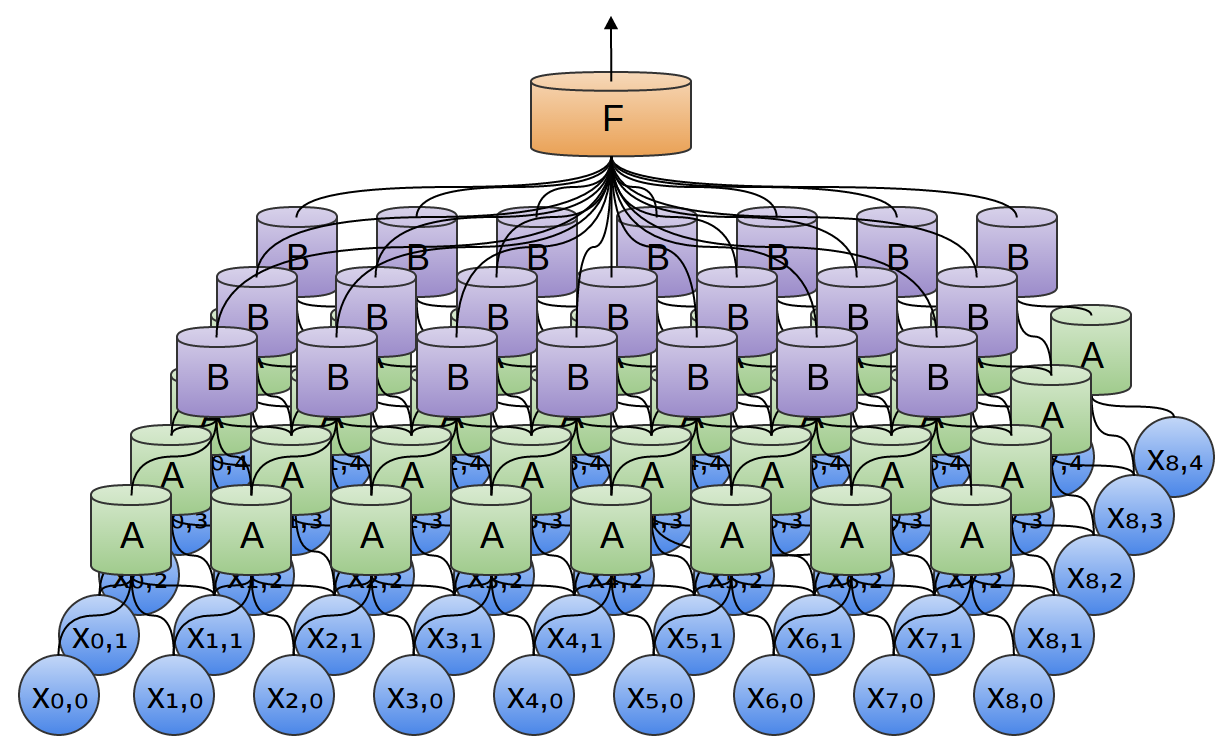
\includegraphics[width=0.4\linewidth]{img/cnn}
	       	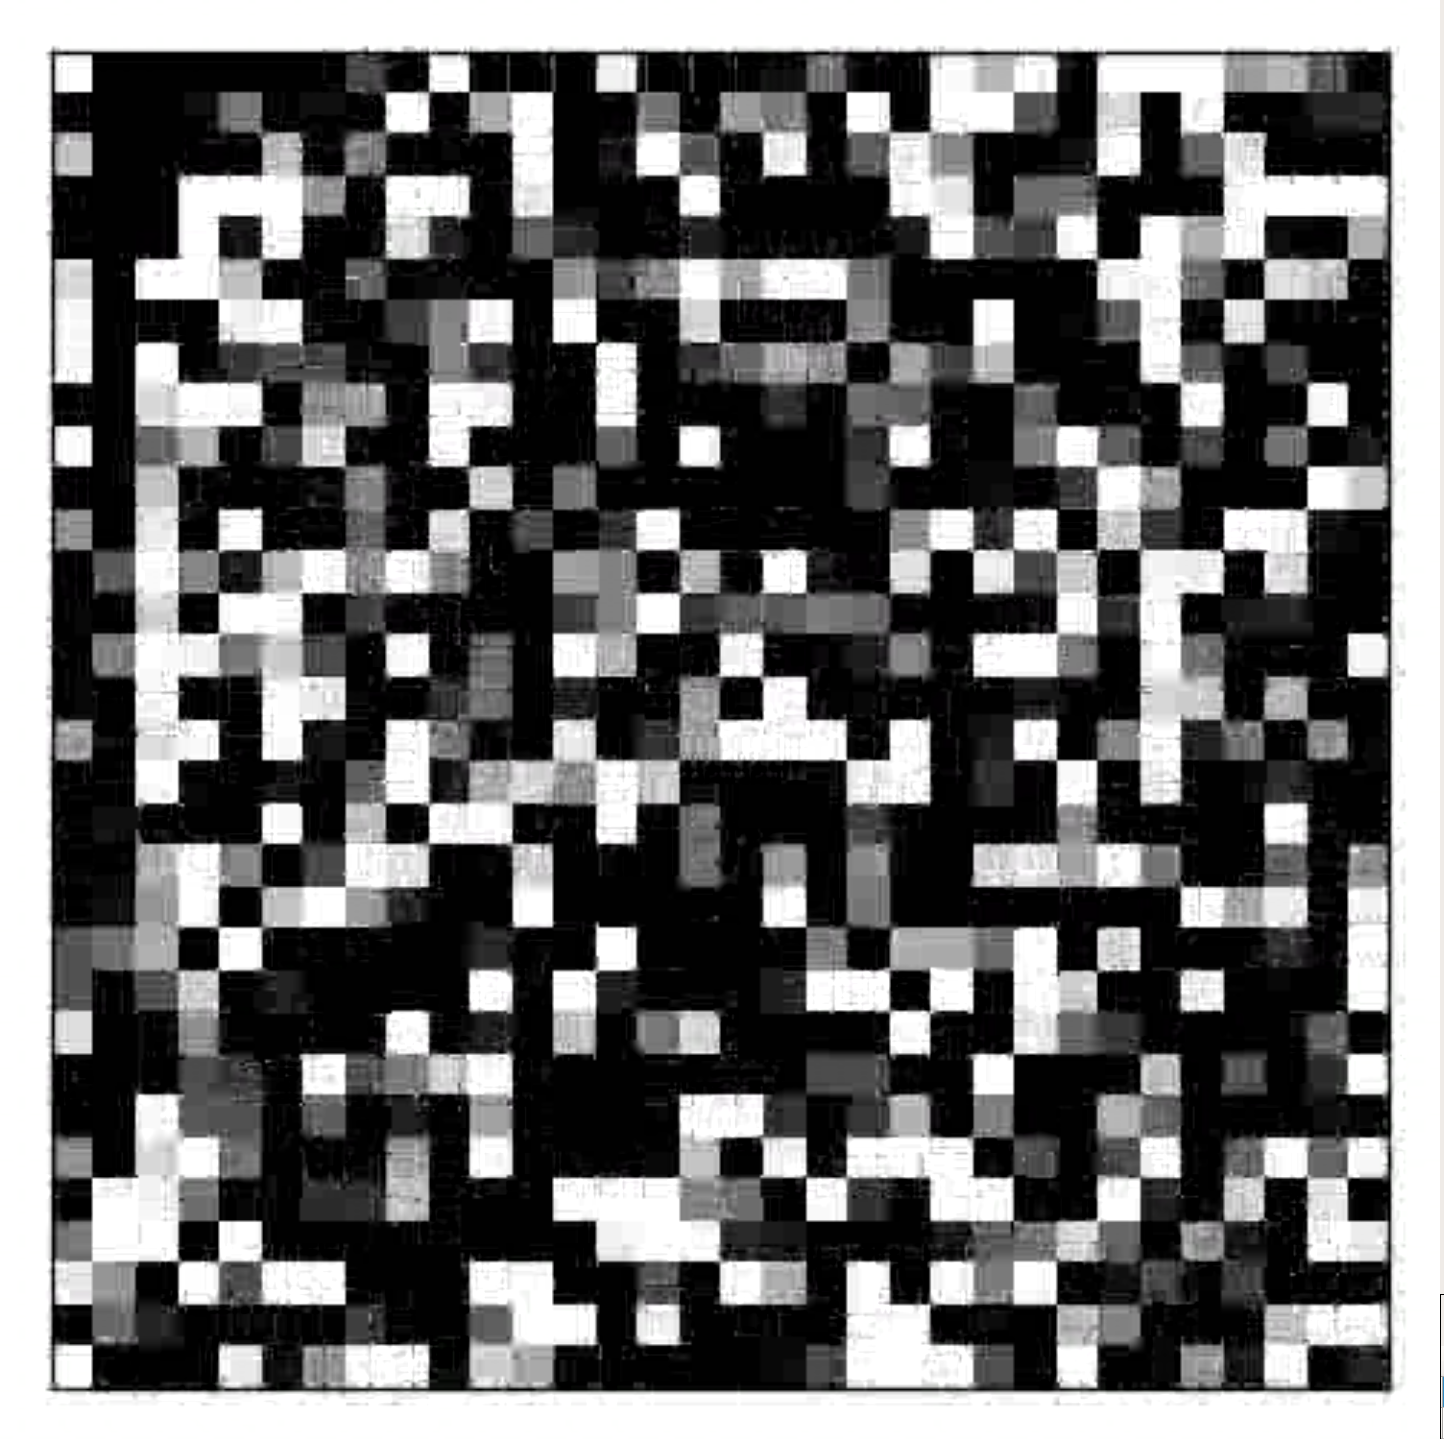
\includegraphics[width=0.4\linewidth]{img/activation}
	       	\caption{Graphical intuiton and arrangement in a traditional convolutional neural network (CNN). In this, A represents a convolution, B an aggregation/downsampling layer such as a softmax, and F is a fully connected neuron.
	       	The right figure is a net trained on MNIST's first layer activation, on an image of all max values. We can see low-level features arising (groups/lines of pixels).}
	       	\label{fig:cnn}
	       \end{figure}
	       \begin{figure}[H]
	       	\centering
	       	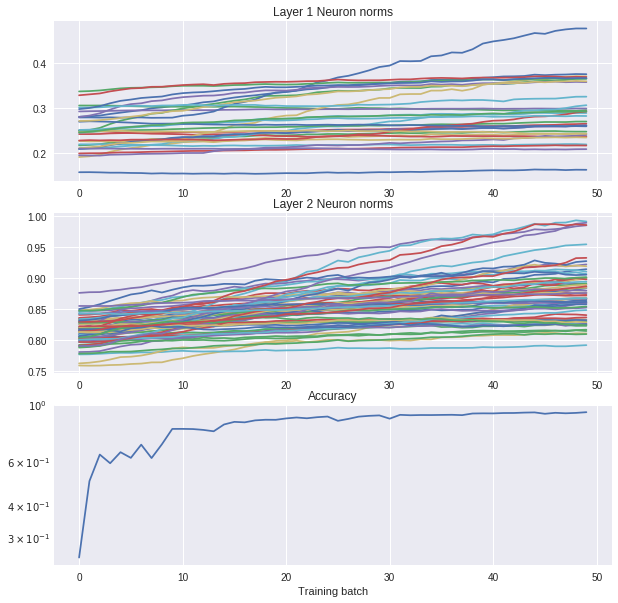
\includegraphics[width=0.6\linewidth]{img/neuron_convergence}
	       	\caption{A depiction of neuron weights in time, as training progresses. We see a strong tend towards limit trend in the norms of the neurons as training progresses.}
	       	\label{fig:neuronconvergence}
	       \end{figure}
        
        \paragraph{Trends in neuron weights} As we view the neurons training, we can see that each has a predetermined distribution across which this is spread. The general widening trend with little reorgainization implies training is done and the network has reached an equilibrium state, with only miniscule incremental gains in performance.
        However, early identification of the asymptotic limit is a possible heuristic that we can use to speed up training.
        Another possible metric is the delta in relative spread across the neuron norms. This manifests in the graph as the ratio of the norms staying roughly equal as the network saturates.
        
    \section*{Performance evaluation of heuristics}
    \paragraph{Baseline performance and success measures}
    In Fig \ref{fig:noisevsnormal}, we can see what a standard no-sleep run looks like, as well as one that has been corrupted by noise. The down-and-right nature of the random noise curve is indicitave of worse performance, and the "fuzz" along the trained network is random noise being injected, and the network compensating with another step of backpropogation.
    Geometrically speaking, it is easy to see what success looks like, relative up-and-left shift of the line.
    \small
    \begin{figure}[H]
    	\centering
    	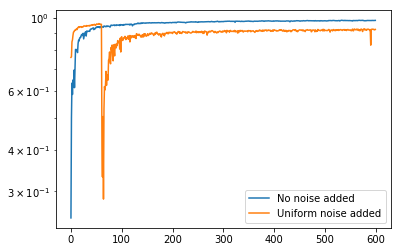
\includegraphics[width=0.6\linewidth]{img/noise_vs_normal}
    	\caption{ Accuracy on the test dataset for number of batches trained. Comparing random noise in the system (uniform in the $-1 \leq x \leq 1$) to the system with no interruptions in backpropogation}
    	\label{fig:noisevsnormal}
    \end{figure}
  \small
  The spike at the beginning deserves mention, as it's a lucky configureation found by chance. We can see it quickly drop off as the opposite happens, a very unlucky sleep operation.
  
  Ideally, we're able to replicate the early boost given by a random sleep (in this case).
    
    
    \section*{Results}
    We started out with an intent to simulate and implement a “sleep” phase for deep learning, during which the model takes no external data and change its weight through some signals in the system. As we researched on sleep in neuroscience\cite{schenck2002rem}, we found that sleep is a very complex behavior that influences mainly the chemical transmission between neurons\cite{ross1984tonic}. It is very hard to generalize and simulate a sleep phase with a single signal neural network system.    
    \begin{figure}[H]
    	\centering
    	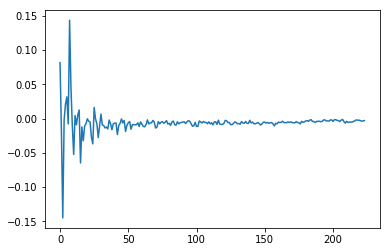
\includegraphics[width=0.4\linewidth]{img/result}
    	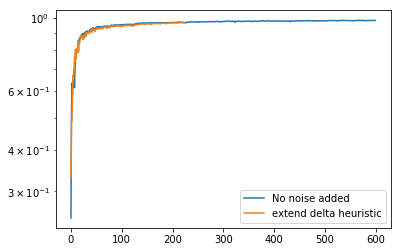
\includegraphics[width=0.4\linewidth]{img/heuristic_result}
    	\caption{Most of our heuristics looked like this (delta)}
    	\label{fig:result}
    \end{figure}
  \begin{figure}[H]
  	\centering
  	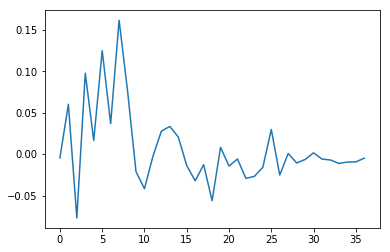
\includegraphics[width=0.4\linewidth]{img/promising}
  	\caption{Some of our heuristics (here \texttt{delta = last\_wts - current\_wts; new\_wts = current\_wts + delta**2}) show promise, improving the training rate by 'boosting' the initial process with a square, that rounds lower as the training cycle goes on.}
  	\label{fig:promising}
  \end{figure}
  
	  \section*{Further work}
	  We still have to try transfer learning with a LSTM-RNN, and more heuristsics are always good to try. Now that we have a toolkit, trying out new things is easy, so we should iterate and try more heuristics. Sleep in a neural network is a challenging thing.
    
    

        
\section*{Bibliography}
\tiny
\bibliographystyle{plain}
\bibliography{cites}


\end{multicols}
\end{document}